\subsection{Custom MLP Network}

\subsubsection{Time Analysis and Compromise}
Initial configuration of the neural network resulted in each iteration of the epoch taking around 0.00015 seconds. On average, a song will have 4 million signal samples which will result in around 40000 iterations per epoch after the subdividing the original signal into chunks. The resulting time per epoch is around 10 hours and is way less than reasonable. The parameters of the neural network were toned down to improve runtimes. The size of each layer was reduced by tenfold and so was the number of layers. This resulted in a rough improvement of 1000 times since the backpropagation algorithm was O($n^2$) on the width of the layer and O(n) on the number of layers. The resulting time per epoch was 30 seconds.\\

\subsubsection{Neural Network Training}
The neural network was trained for a single song as an initial test. The observation was that the cumulative error converged at around 1.9 after 400 epochs, from an initial cumulative error of around 400. When other songs were added to the training set, the cumulative error did not increase by a significant amount. As well, the cumulative error still converged at around 1.9. It was decided at this point that the neural network is in a trained state because the cumulative error did not improve upon further epochs. \\

\subsubsection{Results and Analysis}
The neural network implemented in the previous section experienced premature convergence because the cumulative error did not converge at 0. A music file was inputted into the neural network and its output was observed. The output was observed to contain values between 0.0018 and 0.0026 which meant the neural network decided that there should be no steps for the given music file. This decision was completely unwanted because it is never the case that a music file does not have a single step. As well the max and min of the output array had no observable correlation to either the expected output array or the input array.\\

With the extreme skew of the output, a different approach was used to decide the actual value of the steps output array. The output array from the neural network is used as a probability array. Each element of the array dictates the chance that a step should occur at that time. This probability is further adjusted based on the amount of time that has passed since the last step was detected. This is to account for the fact that steps will never occur too close to each other and that the distance between consecutive steps is always within some threshold.\\\\

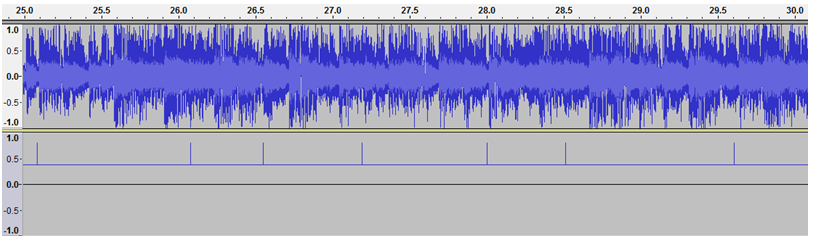
\includegraphics[scale=0.55]{signal_2.png}

Fig x. A visualisation of the input (top) and neural network output with fuzzy logic (bottom).
\\\\
The main reason for the premature convergence of the neural network is the naïve model of input and output that was used. While the sound signal array was well populated, the steps signal array was very sparse. This resulted in an expected output of 0 almost all of the time. As a result, the backpropagation algorithm will try to adjust the network so that the output is as close to 0 as possible to minimize the error. Because the 1s are so sparse, the neural network is unable to retain the learned affected weights from the 1s because they are quickly overwritten by 0s.
Another reason why the training did not go well is because of the nature of the input set. The accompanying steps file for each music file is manually generated by human beings. The human would try their best to assign steps to moments in the song where they perceive a beat or some other musical feature. However, because there is a limit to how fast a person can move their feet in a DDR game, not all beats have steps assigned to them. As a result, the steps file is somewhat of a random subset of the beats of the music file. This randomness in correlation acts to confuse the neural network during training.

\subsubsection{Fuzzy Logic for Input}

After analysis was done, a different way to extract input was attempted to accommodate the sparsity of the steps array. The steps parser was updated so that it may return an array of fuzzified steps. Instead of representing the precise moment of when a step occurred, a bell curve across 100 consecutive samples is used to represent the step, where the peak of the bell curve is the moment the step occurred.

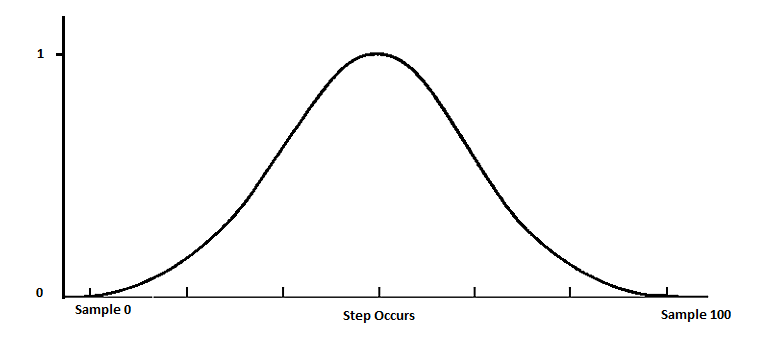
\includegraphics[scale=0.3]{fuzzy.png}

Fig x. Fuzzification of steps in steps array.
This implementation still resulted in premature convergence, with a much larger cumulative error which varies depending on the data set being used. It was conjectured that this methodology is potentially viable perhaps with a different function (instead of a bell curve) with fine-tuned parameters.\\

\subsubsection{Variable Learning Rate}
Another implementation was attempted to accommodate for the sparsity of the steps array. This implementation allowed the neural network to have a variable learning rate depending on the expected output of the current iteration of the epoch. If the iteration contained an expected of output of 1 in its array, the learning rate is increased to accommodate for the rarity of this expected output. This approach resulted in a trained neural net which gave output with more variance (range 0.0025- 0.0102). However, the output still did not reflect either the expected output or the input array.\\

\subsection{Keras MLP Network}

The results of the neural network built using Keras had inconclusive findings like our custom network. Like the custom network, this model was trained with 300 songs and each's beat information.

\subsubsection{Accuracy}

Fitting songs to the already trained model yielded accuracy $30\%$ to $60\%$. This accuracy represents the probability that a given timeframe was classified as a beat or not a beat correctly. This percentage of error  is too high for this model to be used for production systems.

\subsubsection{Error}

This model used a stochastic gradient descent algorithm with the mean-squared error function. When fitting songs to the trained model, error varied in the 0.3 to 0.7 range. 

\subsubsection{Graphs}

Using the Keras network model, we plotted the graphs indicate when our model predicted beats would occur vs. where beats actually did occur 

\includegraphics[scale=1.0]{kmp_gd.eps}

The X axis represents the timeframe at which a beat occurred. Note, these are not discrete times but sequential timeframes. The blue lines indicate when beats actually occur and the red lines indicate when the model predicted beats would occur. The Y-scale is irrelevant. Observe how the model predicts a beat for many adjacent timeframes. A correct model would have impulses for a much smaller range of timeframes, similar to how the beats actually occur.

\includegraphics[scale=1.0]{kmp_gd.png}

This graph plots the amplitude values for the given song for all of its timeframers. This is what the raw data for our model looks like when visualized. Observe that the blue and orange lines represent different channels of a wavelet file.


\subsection{Summary}
The main initial approach had major shortcomings and so did its improved versions. The failures of these approaches can be easily attributed to the naivety of the assumptions made about the data. The overarching idea is that raw data is not what humans use to generate steps file or beats and that they should not be used by machines either because the goal is to simulate human steps generation. A more advanced form of feature extraction is necessary as well as possible other changes to the neural network type and parameters being used.